\section{Message Passing Example}

\definecolor{darkgreen}{rgb}{0,0.6,0}



\begin{frame} \frametitle{Inference}
	%\begin{textblock}{14}(0.5,3)
	\begin{enumerate}
		\item<1-> initialization of the clique potentials $f_k(\mathcal X_k)$
			\only<1>{ \begin{itemize}
				\item in the order established by 
					topological sorting	\\(e.g.
					$A \to B \to C \to E \to D \to F$) \\
					
					\vspace{2mm}
					{\small\begin{tabular}{|c|c|c|c|}
					\hline 
					$f_1(A,B,C)$ & $f_2(B,C,E)$ & $f_3(B,D)$ & $f_4(B,E,F)$ \\
					\hline 
					%\hline
					%$P(A,B,C)$ & $\frac{P(B,C,E)}{P(B,C)}$ & $\frac{P(B,D)}{P(B)}$ 
					%	& $\frac{P(B,E,F)}{P(B,E)}$ \\
					%\hline
					$P(C|A)\,P(B|A)\,P(A)$ & $P(E|C)$ & $P(D|B)$ & $P(F|B,E)$ \\
					\hline
					\end{tabular} }
			\end{itemize} }
		\only<1>{\vspace{4mm}
			{\small 
			\begin{equation} \slidesonly{\hspace{-4mm}}
				P(A,B,C,D,E,F) \;\;=\;\; 
				P(A) \, P(B|A) \, P(C|A) \, P(D|B) \, P(E|C) \, P(F|B,E) 
			\end{equation}
			\slidesonly{\vspace{-10mm}}
			}
		}
		\item<2-> modification of the clique potentials by the observed evidence
			\only<2>{\begin{itemize}
				\item for each observation $Y=y^*$ find {\em one} 
					$f_k$ with $Y \in \mathcal X_k$
				\item add a node 
					{\footnotesize $
						f_k(Y) = 
						\left\{\begin{array}{c} 
							1, \; Y=y^* \\[-1mm]
							0, \; Y \neq y^* 
						\end{array}\right.
					$}
				\item example: ${\boxed {D=d^*}}$ and ${\boxed {E=e^*}}$ 
			\end{itemize} }
		\vspace{2mm}
		\item<3-> message passing 
			\only<3>{\begin{itemize}
				\item begin {\color{red}``request'' pass} 
					from arbitrary node $N$,\\e.g.~${\boxed {D=d^*}}$ or ${\boxed{f_1}}$ or \ldots
				\item wait for all message of {\color{blue}``collect'' pass} 
							to return
				\item send last {\color{darkgreen}``distribute'' pass} from $N$
				\itR  all marginals are computed simultaneously
			\end{itemize}}
		\vspace{2mm}
		\item<4-> calculate marginals from messages
			\only<4>{ \small
				\begin{equation}
					P(C, \,D = d^*, E = e^*) 
						\quad=\quad \sum_{b}{} \;
							{\color{blue}\mu_{f_1 \to BC}(b,C)} \cdot 
							{\color{darkgreen} \mu_{f_2 \to BC}(b,C)} 
				\end{equation}
			}
		\item<5-> normalization yields conditional marginals
			\only<5>{ \small
				\begin{equation}
					P(C\, | D = d^*, E = e^*) = \alpha \, \underbrace{P(C, \,D = d^*, E = e^*)}_{\tilde P(C)}, \slidesonly{\quad\quad}\qquad \alpha = \frac{1}{\sum_c \tilde P(c)}
				\end{equation}
			}
	\end{enumerate}	
	%\end{textblock}
	
	%\begin{textblock}{15}(1.5,9.5)
	
	\slidesonly{\vspace{-10mm}}
		\begin{minipage}{12cm}
			\begin{minipage}{4cm}
				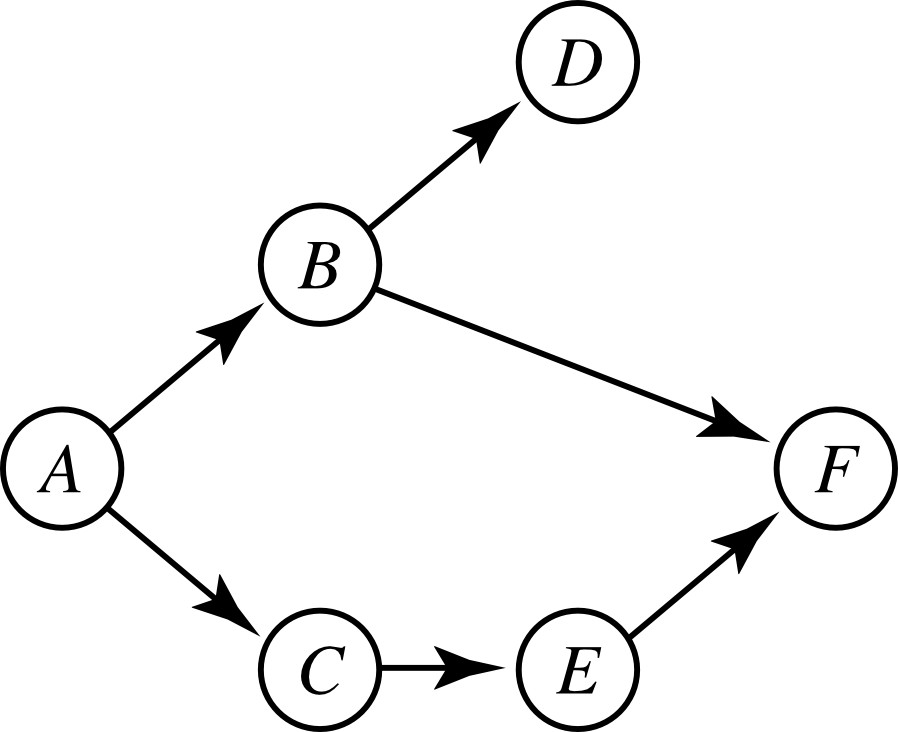
\includegraphics[width=3cm]{img/graph_example_dag.jpg}
				\mode<article>{
				\captionof{figure}{Original DAG}
				}
			\end{minipage}
			\begin{minipage}{7cm}
			\mode<presentation>{
				\includegraphics<1>[height=3cm]%
					{img/graph_example_junction_tree_init_v2.pdf}
				%\mode<article>{
				%\captionof{figure}{Corresponding junction tree with clique potentials}
				%}
				}
				\includegraphics<2>[height=3.5cm]%
					{img/graph_example_junction_tree_evidence_v2.pdf}
				\mode<article>{
				\captionof{figure}{Adding clique potentials for observed variables to the corresponding junction tree}
				}
				\includegraphics<3->[height=3.5cm]%
					{img/graph_example_junction_tree_messages_v2_noextra}
				\mode<article>{
				\captionof{figure}{Flow during the 3 passes.}
				}
			\end{minipage}
		\end{minipage}
	%\end{textblock}
\end{frame}

\begin{frame}{Only}\frametitle{Message passing exercise}

\mode<presentation>{

\placeimage{9.}{0.8}{img/graph_example_junction_tree_messages_v2_noextra}{height=2.5cm}

\begin{block}{sum-product}
\slidesonly{\vspace{-4mm}}
\begingroup
\small
	\begin{align}
		\mu_{X_m \to f_s}(X_m) &\;:=&&\kern-4ex
			\kern-3ex\prod_{l \in \text{neighbor}(X_m) \setminus\{f_s\}}\kern-3ex
			\mu_{f_l \to X_m}(X_m) \tag{product}\\[1mm] 
		\mu_{f_s \to X_i}(X_i) &\;:=&&\kern-3ex 
			\sum_{x_m, \ldots, x_M}\kern-2ex f_s(X_i, x_m,\ldots, x_M) 
			\kern-5ex\prod_{k \in \text{neighbor}(f_s)\setminus\{X_i\}}\kern-5ex 
			\mu_{X_k \to f_s}(x_k) 
			\only<1>{\nonumber\hspace{10mm}}
			\only<2>{\tag{sum}}
	\end{align}
\endgroup
    \end{block}
    }
    
Define the messages by applying the sum-product-algorithm\notesonly{ from \eqref{eq:sumproduct}}:

\begingroup
\footnotesize
\begin{enumerate}
 \item<only@1> Define potentials for observed variables (in this case $D=d^*$ and $E=e^*$):
 \begin{enumerate}[\notesonly{(}a\notesonly{)}]
 \item $f_5(D) = 
						\left\{\begin{array}{c} 
							1, \; D=d^* \\[-1mm]
							0, \; D \neq d^* 
						\end{array}\right.$
 \item $f_6(E) = 
						\left\{\begin{array}{c} 
							1, \; E=e^* \\[-1mm]
							0, \; E \neq e^*
						\end{array}\right.$
 \end{enumerate}
 \item<only@1> Select root (e.g. $f_{5}$), doesn't matter much. \notesonly{It will affect the order in which we the messages are defined (either in the collect or in the distribute pass).}
 \item<only@1-5> \textcolor{blue}{collect} (start at leaf node): \slidesonly{\only<1>{\textbf{(see blackboard)}}}
 \begin{enumerate}[\notesonly{(}a\notesonly{)}]
  \item<only@2> `branch on the right':
  \begin{enumerate}[\notesonly{(}i\notesonly{)}]
  \item $\msg{f_{1}}{B,C}(B,C) := \sum_{a} f_{1}(a,B,C) \overbrace{\hcancel{\prod_{k \in \text{neigh.}(f_s)\setminus\{X_i\}}\kern-5ex 
			\mu_{X_k \to f_s}(X_k)}}^{\text{no other neighbors}}$
  \item $\msg{B,C}{f_{2}}(B,C) := \msg{f_{1}}{B,C}(B,C) = \sum_{a} f_{1}(a,B,C)$
  \end{enumerate}
  \item<only@3> `top branch':
  \begin{enumerate}[\notesonly{(}i\notesonly{)}]
  \item $\msg{f_{4}}{B,E}(B,E) := \sum_{f} f_{4}(B,E,f)$
  \item $\msg{B,E}{f_{2}}(B,E) := \msg{f_{4}}{B,E}(B,E) = \sum_{f} f_{4}(B,E,f)$
  \end{enumerate}
  \item<only@4> `bottom branch':
  \begin{enumerate}[\notesonly{(}i\notesonly{)}]
  \item $\msg{f_{6}}{E}(E) := f_{6}(E)$
  \item $\msg{E}{f_{2}}(E) := \msg{f_{6}}{E}(E) = f_{6}(E)$
  \end{enumerate}
  \item<only@5> `left branch':
  \begin{enumerate}[\notesonly{(}i\notesonly{)}]
  \item $\msg{f_{2}}{B}(B) := \sum_{c,e} f_{2}(B,c,e) \cdot \msg{E}{f_{2}}(e) \cdot \msg{B,E}{f_{2}}(B,e) \cdot \msg{B,C}{f_{2}}(B,c)$
  \item $\msg{B}{f_{3}}(B) := \msg{f_{2}}{B}(B)$
  \item $\msg{f_{3}}{D}(D) := \sum_{b} f_{3}(b,D) \cdot \msg{B}{f_{3}}(b)$
  \item $\msg{D}{f_{5}}(D) := \msg{f_{3}}{D}(D)$
  \end{enumerate}
 \end{enumerate}
 \item<only@6->  \textcolor{darkgreen}{distribute} (start at root node):
 \begin{enumerate}[\notesonly{(}a\notesonly{)}]
  \item<only@7> go right:
  \begin{enumerate}[\notesonly{(}i\notesonly{)}]
    \item $\msg{f_{5}}{D}(D) := f_{5}(D)$
    \item $\msg{D}{f_{3}}(D) := \msg{f_{5}}{D}(D) = f_{5}(D)$
    \item $\msg{f_{3}}{B}(B) := \sum_{d} f_{3}(B,d) \cdot \msg{D}{f_{3}}(d)$  
    \item $\msg{B}{f_{2}}(B) := \msg{f_{3}}{B}(B)$    
    \end{enumerate}
  \item<only@8-9> go further to the right:
  \begin{enumerate}[\notesonly{(}i\notesonly{)}]
  \item $\msg{f_{2}}{B,C}(B,C) := \sum_{e} f_{2}(B,C,e) \cdot \msg{E}{f_{2}}(e) \cdot \msg{B,E}{f_{2}}(B,e) \cdot \msg{B}{f_{2}}(B) $
  \item $\msg{B,C}{f_{1}}(B,C) := \ldots$ 
  \end{enumerate}
  \item<only@9> go up: $\ldots$
  \item<only@9> go down: $\ldots$
  \end{enumerate}
  \item<only@10> calculate marginals:
  \begin{enumerate}[\notesonly{(}a\notesonly{)}]
  \item \begin{align}
					P(C, \,D = d^*, E = e^*) 
						\;\; =& \;\; \sum_{b}{} \;
							{\color{blue}\mu_{f_1 \to BC}(B,C)} \cdot 
							{\color{darkgreen} \mu_{f_2 \to BC}(B,C)} 
		\end{align}
  \item other queries you are interested in $\ldots$
  \end{enumerate}
  \item<only@11> normalize to compute conditional marginals:
  \begin{enumerate}
  \item[]
  \slidesonly{\vspace{-3mm}}
   \begin{align}
            P(C\, | D = d^*, E = e^*) &= \alpha \, \underbrace{P(C, \,D = d^*, E = e^*)}_{\tilde P(C)},\\
            \text{where} \;\; \alpha &= \frac{1}{\sum_c \tilde P(c)}
		\end{align}
  \end{enumerate}
  
\end{enumerate}
 \endgroup
\end{frame}



